\section{User Modeling}
\label{sec:modeling}

The term \emph{user modeling} (\smallcaps{UM}) lacks a strict definition. 
Broadly speaking, when an application is adapted in some way based on what the system knows about its users, we have user modeling. 
From predictive modeling methods in machine learning, 
to how interface design is influenced by personalization, the field covers a lot of ground. 

It is important to differentiate between adapting the interface of an application and the content of an application. 
Many user modeling methods strive to personalize the interface itself, e.g. menus, buttons and control elements 
(e.g. \cite{Jameson2009, Fischer2001}. 
Adapting the application content, on the other hand, means changing how and what content is displayed.
For instance, interface adaption might mean changing the order of items in a menu, while content 
adaption might mean changing the order and emphasis of results in a web search interface
(e.g. \cite{Xu2008, Qiu2006, Rhodes2000}).

In this thesis, we are interested in adapting the \emph{content} of an application.
We believe the information overload problem often stems from a mismatch between presented content and desired content. 
Examples of adaptive content include:

\begin{itemize*}
  \item Suggesting interesting items based on previous activity.
  \item Reorganizing or filtering content based on predicted user relevance.
  \item Translating content based on a user's geographical location.
  \item Changing the presentation of content to match personal preferences or abilities.
  \item Personalizing search results based on previous queries and clicks.
\end{itemize*}

The fields of Artificial Intelligence (AI) and Human-Computer Interaction (HCI) share a common goal solving information overload through user modeling. 
However, as described by \cite[p.6]{Lieberman2009}, they have different approaches and their efforts are seldom combined. 
While AI researchers often view contributions from HCI as trivial cosmetics, the HCI camp
tends to view AI as unreliable and unpredictable --- surefire aspects of poor interaction design.

In AI, user modeling refers to algorithms and methods that infer knowledge about a user based on past interaction 
(e.g. \cite{Pazzani2007, Smyth2007, Alshamri2008, Resnick1994}).
By examining previous actions, predictions can be made of how the user will react to future information. This new knowledge is then embedded in a model of the user, which can predict future actions and reactions. 
For instance, an individual user model may predict how interesting an unseen article will be to a user, based on previous feedback on similar articles or the feedback of similar users.

HCI aims to meet user demands for interaction. 
User modeling plays a crucial role in this task. 
Unlike the formal user modeling methods of AI, user models in HCI are often cognitive approximations, manually developed by researchers to describe different types of users 
(e.g. \cite{Fischer2001, Jameson2009, Cato2001}).
These models are then utilized by interaction designers to properly design the computer interface based on a models predictions of its user's preferences.
\cite{Totterdell1990} describes user modeling in interaction design as a collection of deferred parameters: 

\begin{blockquote}
  ``The designer defers some of the design parameters such that they can be selected or 
  fixed by features of the environment at the time of interaction [...] 
  Conventional systems are special cases of adaptive systems in which the parameters have been pre-set.'' 
\end{blockquote}

This thesis is concerned with the AI approach to user modeling, and in particular, the use of \emph{recommender systems} (RSs).

\subsection{Interface Autonomy}

\begin{figure}[t]
  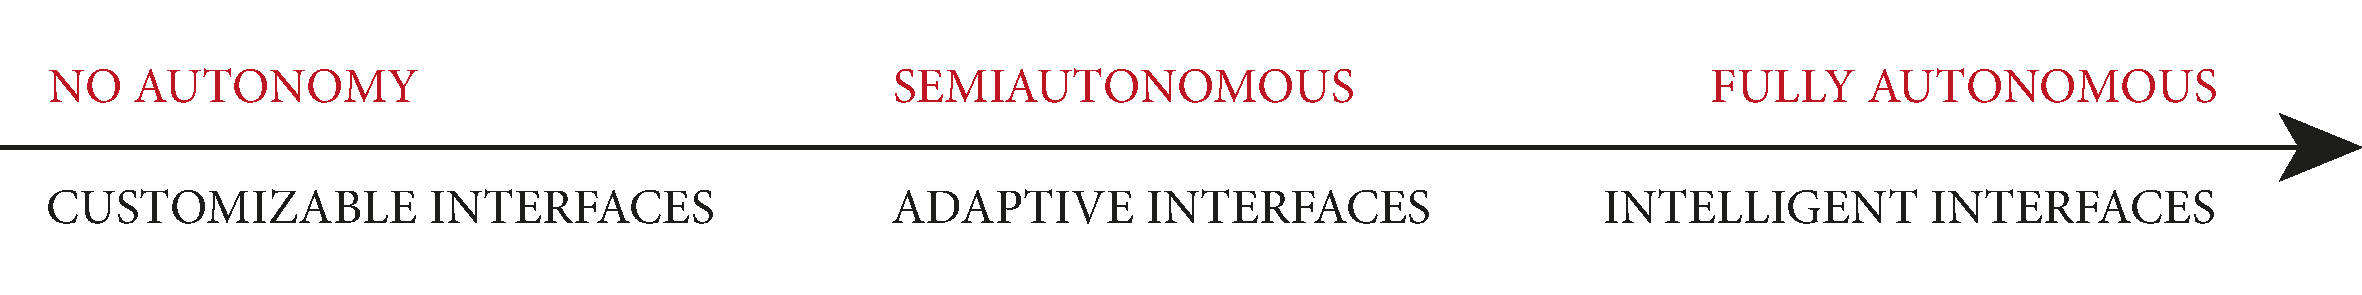
\includegraphics[width=\textwidth]{../graphics/autonomy.pdf}
  \caption[Levels of Interface Autonomy]{
    Levels of Interface Autonomy:
    Interfaces range from those only customizable by the user, 
    to intelligent systems takes the initiative on their own accord.
  }
  \label{fig:autonomy}
\end{figure}

Using AI to adapt an interface raises important questions with regard to usability, privacy and usefulness.
These questions are rooted in the autonomy expressed by each interface.
An autonomous interface is one that takes initiatives on its own, regardless of whether the user has asked for it \cite[p.2]{Lieberman}. 
Naturally, any application that automatically personalizes its content will be autonomous to some degree.

Adaptive interfaces can be classified into increasing order of autonomy (see Figure \ref{fig:autonomy}). 
At the order of least autonomous systems, we have \emph{customizable interfaces}. 
These are interfaces that the user may customize themselves, but that do not take the initiative or change anything without explicit user action. 
For example, an interface might have a settings panel where users can change the order of items in a menu.

At the next level of autonomy, we have \emph{adaptive interfaces} that suggest to the user possible changes or actions that might be beneficial. For example, an email application could suggest which folder an email should be moved to.
At the most autonomous level, \emph{intelligent interfaces} implicitly and automatically customize the interface or content based on passive observation of the user. 
This could for instance entail automatic filing of emails based on content classification and data mining of previous user actions with similar messages.

An application that personalizes content automatically will fall somewhere in the two last categories and present either an adaptive or intelligent interface, 
depending on the extent and transparency of its autonomy.

In this thesis, we are only interested in fully autonomous, intelligent interfaces.
We will create a system that implicitly, and without any effort from each user,
can adapt the content of an application based on previous behavior.
Other examples of such implicit user modeling include \cite{Qiu2006}, \cite{Shen2005} and \cite{Carmel2009}.

As our goal is to adaptively combine different RSs based on each user and item,
we shall now describe what makes a recommender system, and introduce some of the many algorithms they employ.
